\documentclass[boxes,pages]{homework}

\name{Nate Stemen}
\studentid{20906566}
\email{nate.stemen@uwaterloo.ca}
\term{Fall 2020}
\course{Numerical Analysis}
\courseid{AMATH 740}
\hwnum{2}
\duedate{Fri, Sep 25, 2020 5:00 PM}

\hwname{Assignment}
% \problemname{Exercise}
%\solutionname{(Name)}


\usepackage{physics}
\usepackage{cleveref}
\usepackage{listings}
\usepackage{xcolor}
\usepackage{graphicx}
\usepackage{caption}
\usepackage{subcaption}

\definecolor{codegreen}{rgb}{0,0.6,0}
\definecolor{codegray}{rgb}{0.5,0.5,0.5}
\definecolor{codepurple}{rgb}{0.58,0,0.82}
\definecolor{backcolour}{rgb}{0.95,0.95,0.92}

\lstdefinestyle{mystyle}{
  backgroundcolor=\color{backcolour},
  commentstyle=\color{codegreen},
  keywordstyle=\color{magenta},
  numberstyle=\tiny\color{codegray},
  stringstyle=\color{codepurple},
  basicstyle=\ttfamily\footnotesize,
  breakatwhitespace=false,
  breaklines=true,
  captionpos=b,
  keepspaces=true,
  numbers=left,
  numbersep=5pt,
  showspaces=false,
  showstringspaces=false,
  showtabs=false,
  tabsize=2
}
\lstset{style=mystyle}

\newcommand{\tpose}[1]{#1^\intercal}
\newcommand{\inv}[1]{#1^{-1}}


\begin{document}

\problemnumber{3}

\begin{problem}
2D model problem.
\end{problem}

\begin{solution}
	First a spy plot.
	\begin{figure}[h]
		\centering
		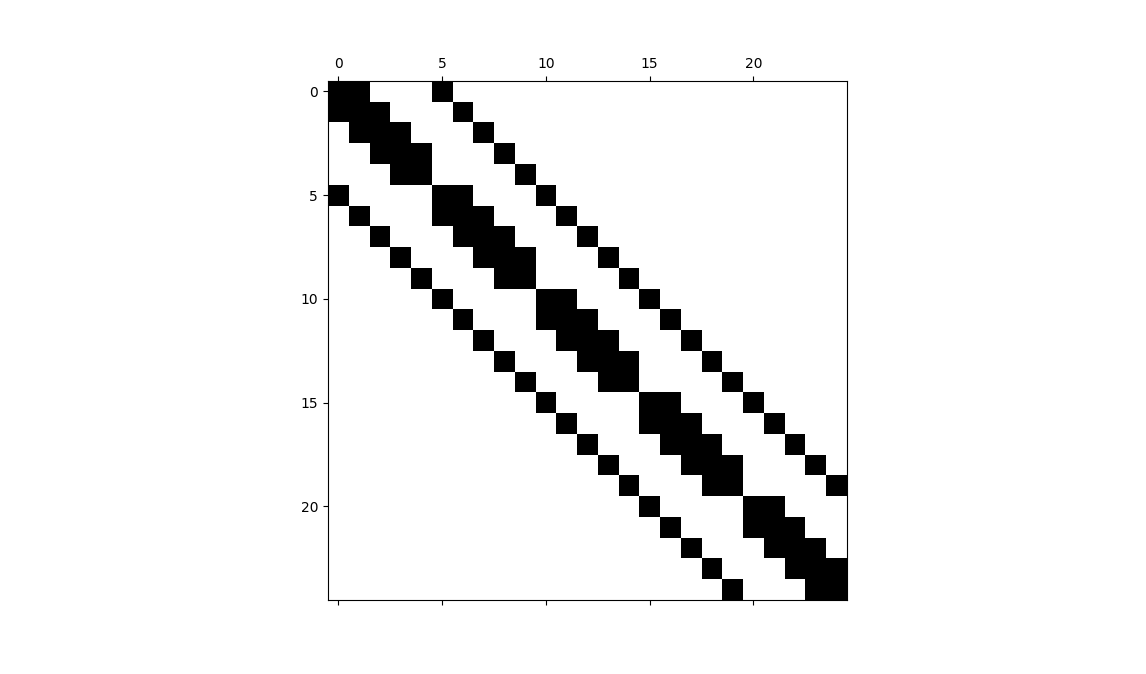
\includegraphics[width=0.9\textwidth]{problemThree/spy.png}
		\caption{Spy plot for 2D Laplacian Matrix with $N = 5$}
	\end{figure}

	Here's the code from \verb|build_laplace_2d.py|.
	\lstinputlisting[language=Python]{problemThree/build_laplace_2d.py}
	\subsubsection*{Laplace's equation}
	Below are the exact and approximate solutions along with the error. Note the vertical axis has changed quite a bit for the error.
	\begin{figure}[h]
		\centering
		\begin{subfigure}{.5\textwidth}
			\centering
			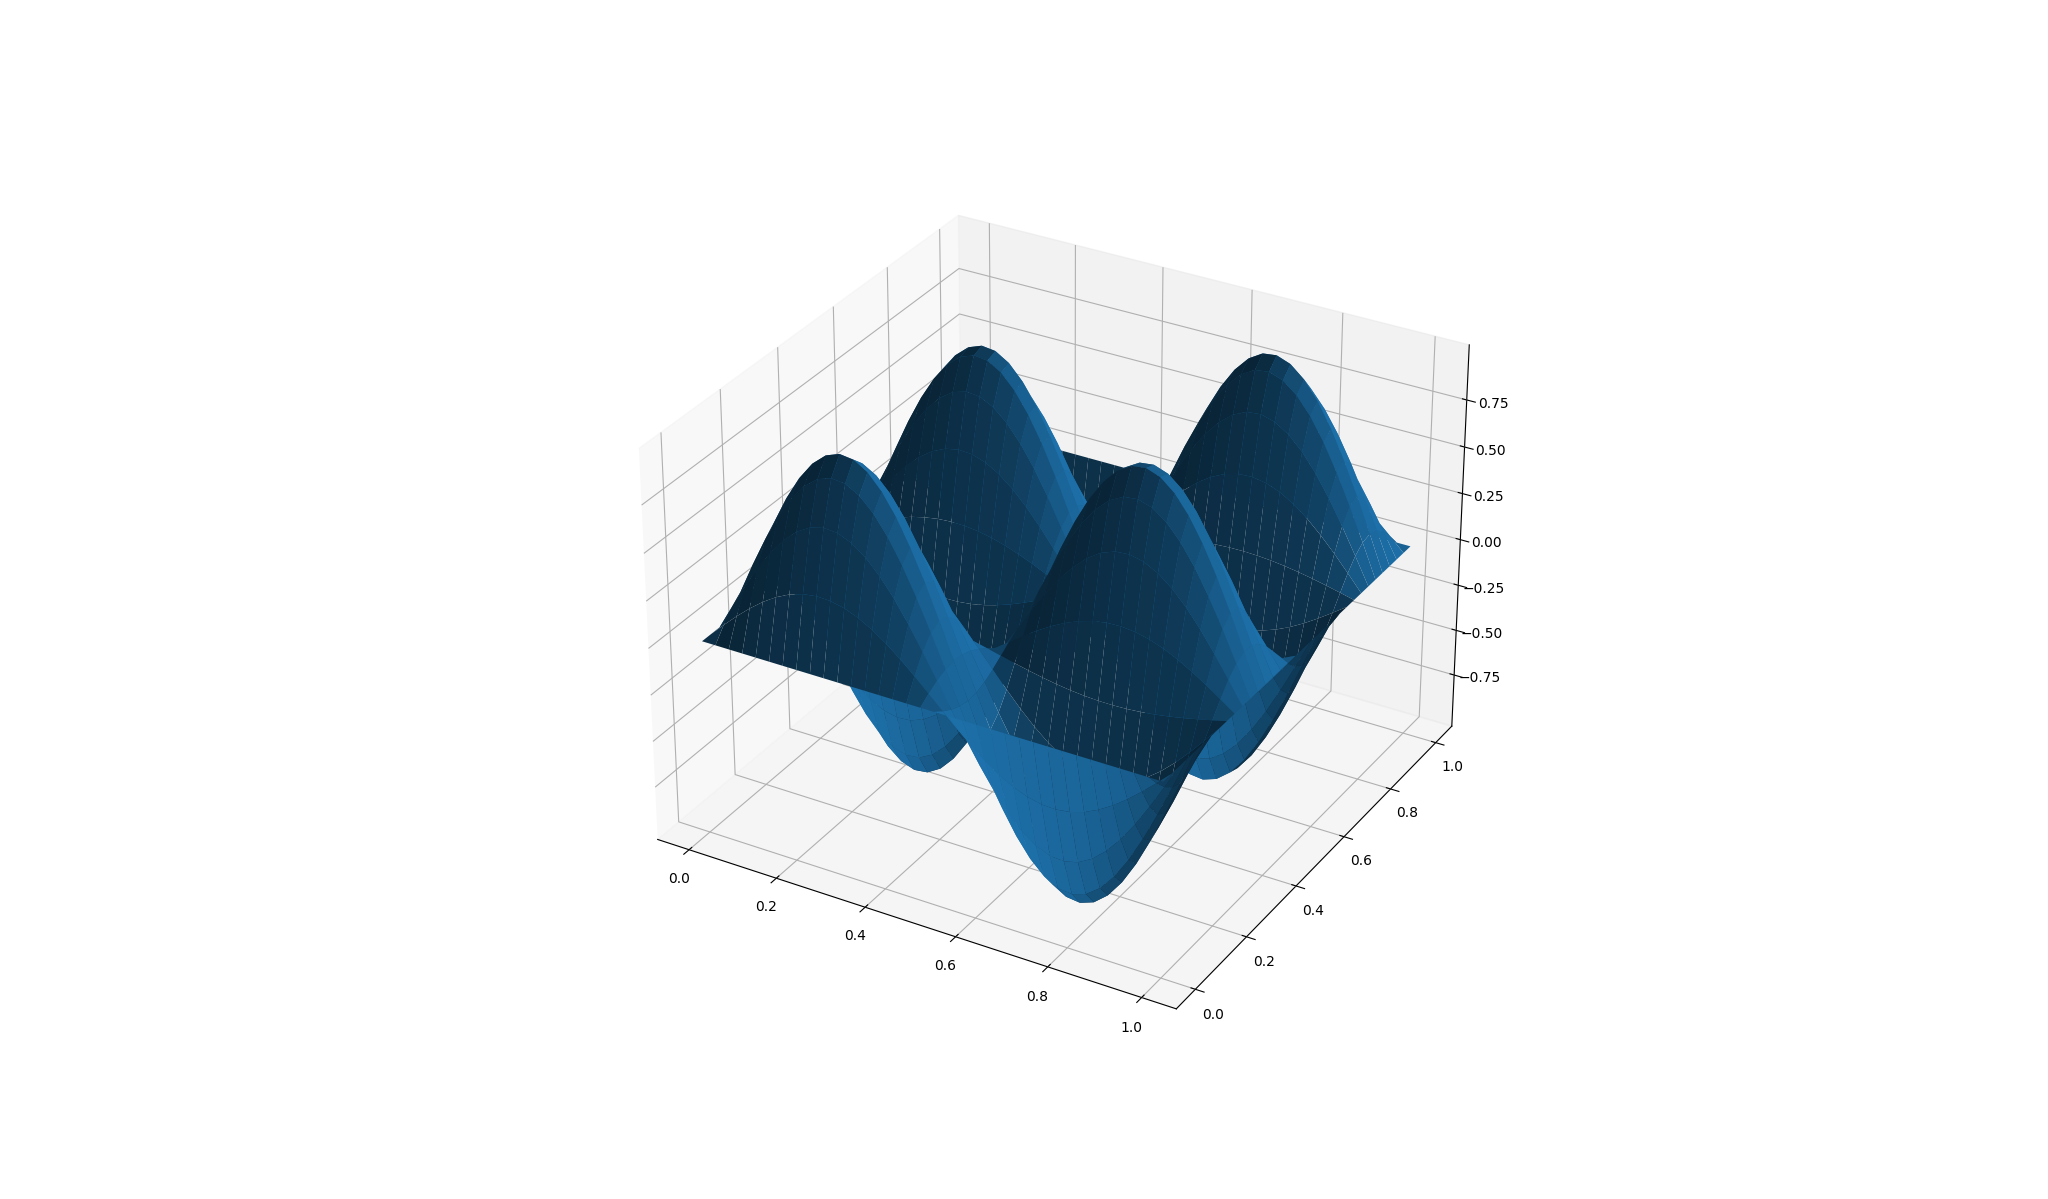
\includegraphics[width=.9\linewidth]{problemThree/exact.png}
			\caption{Exact solution}
			\label{fig:sub1}
		\end{subfigure}%
		\begin{subfigure}{.5\textwidth}
			\centering
			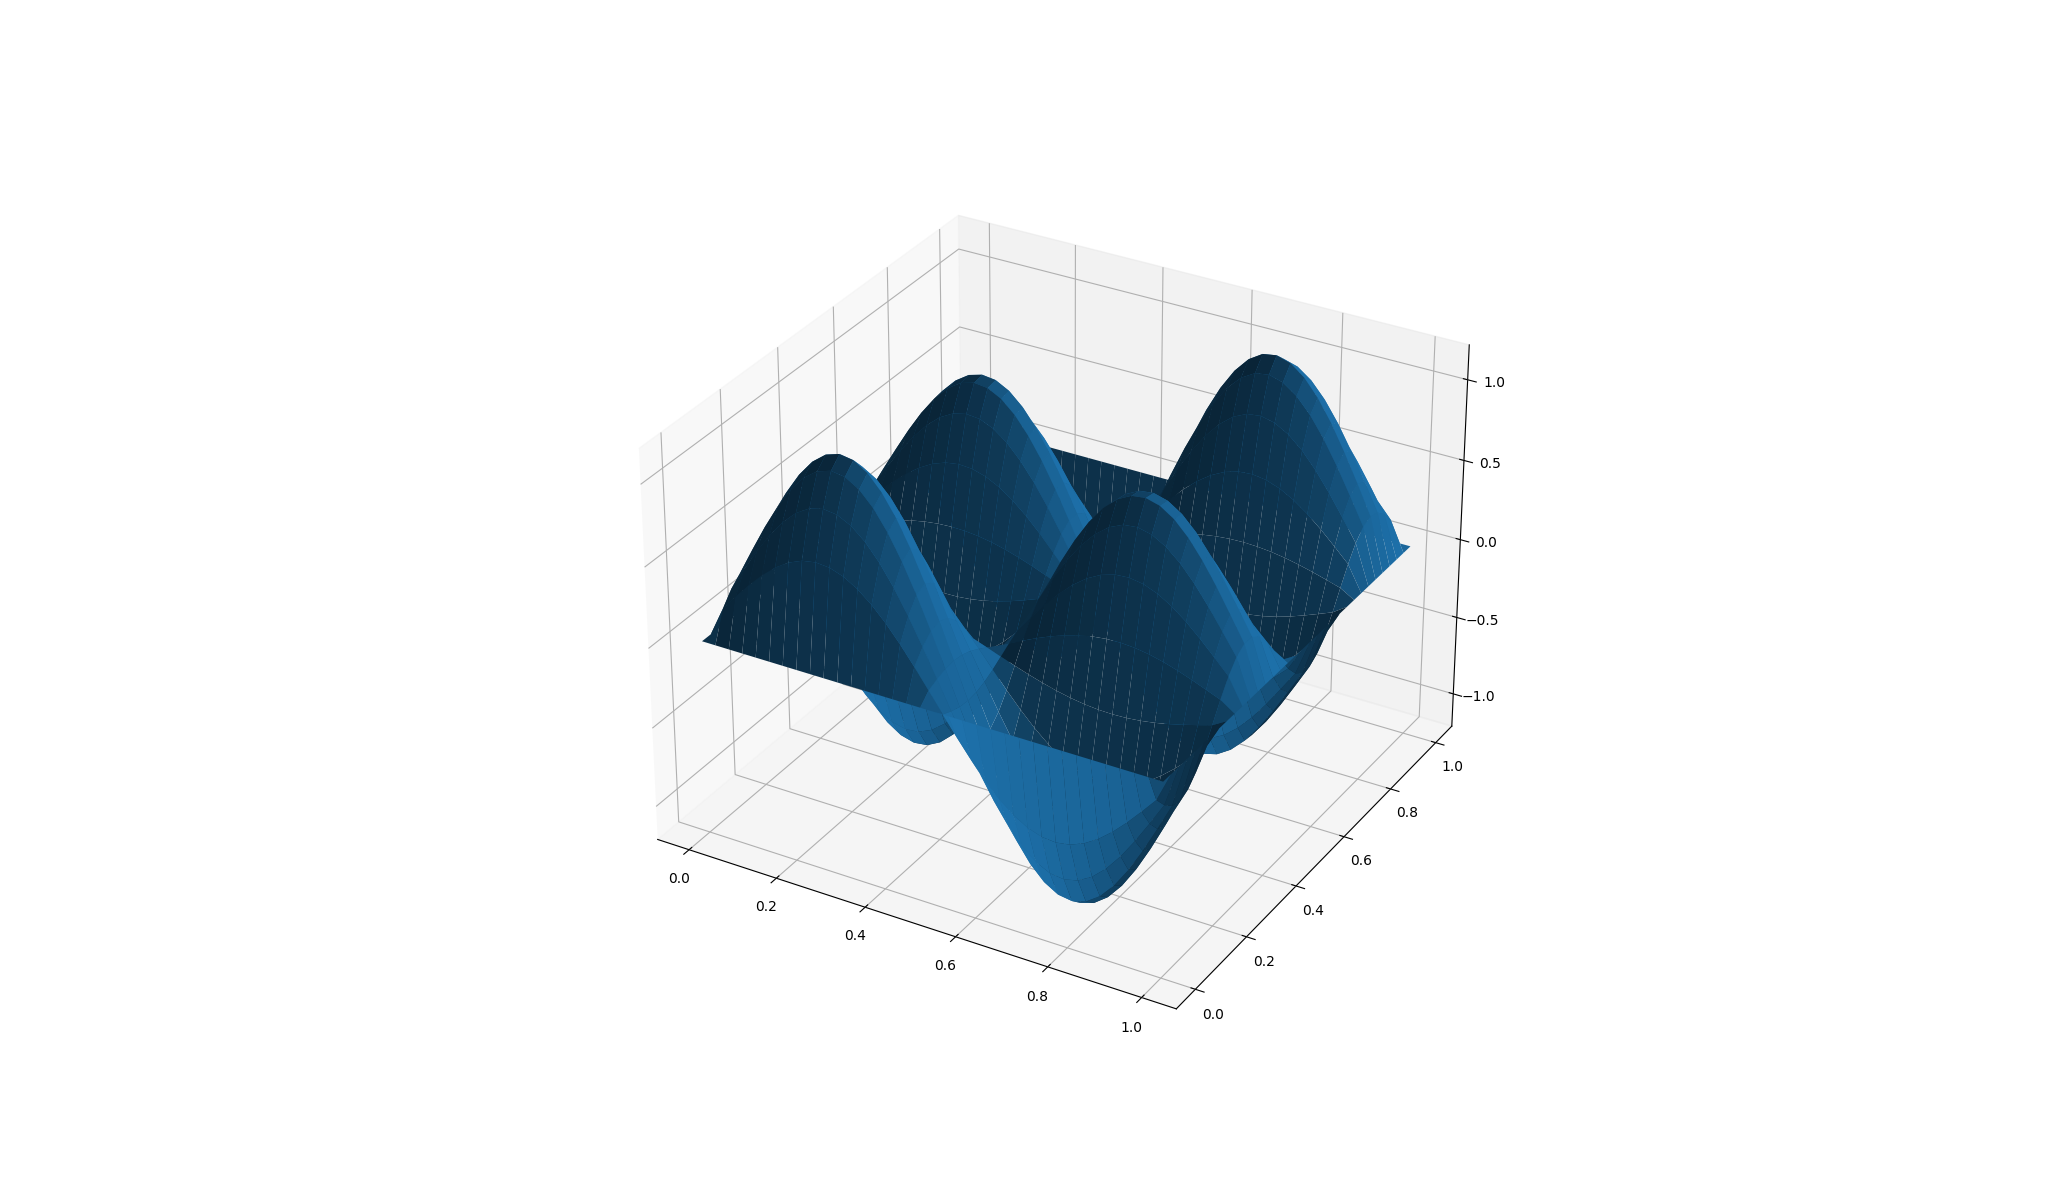
\includegraphics[width=.9\linewidth]{problemThree/solution.png}
			\caption{Approximate solution}
			\label{fig:sub2}
		\end{subfigure}
	\end{figure}
	\begin{figure}[h]
		\centering
		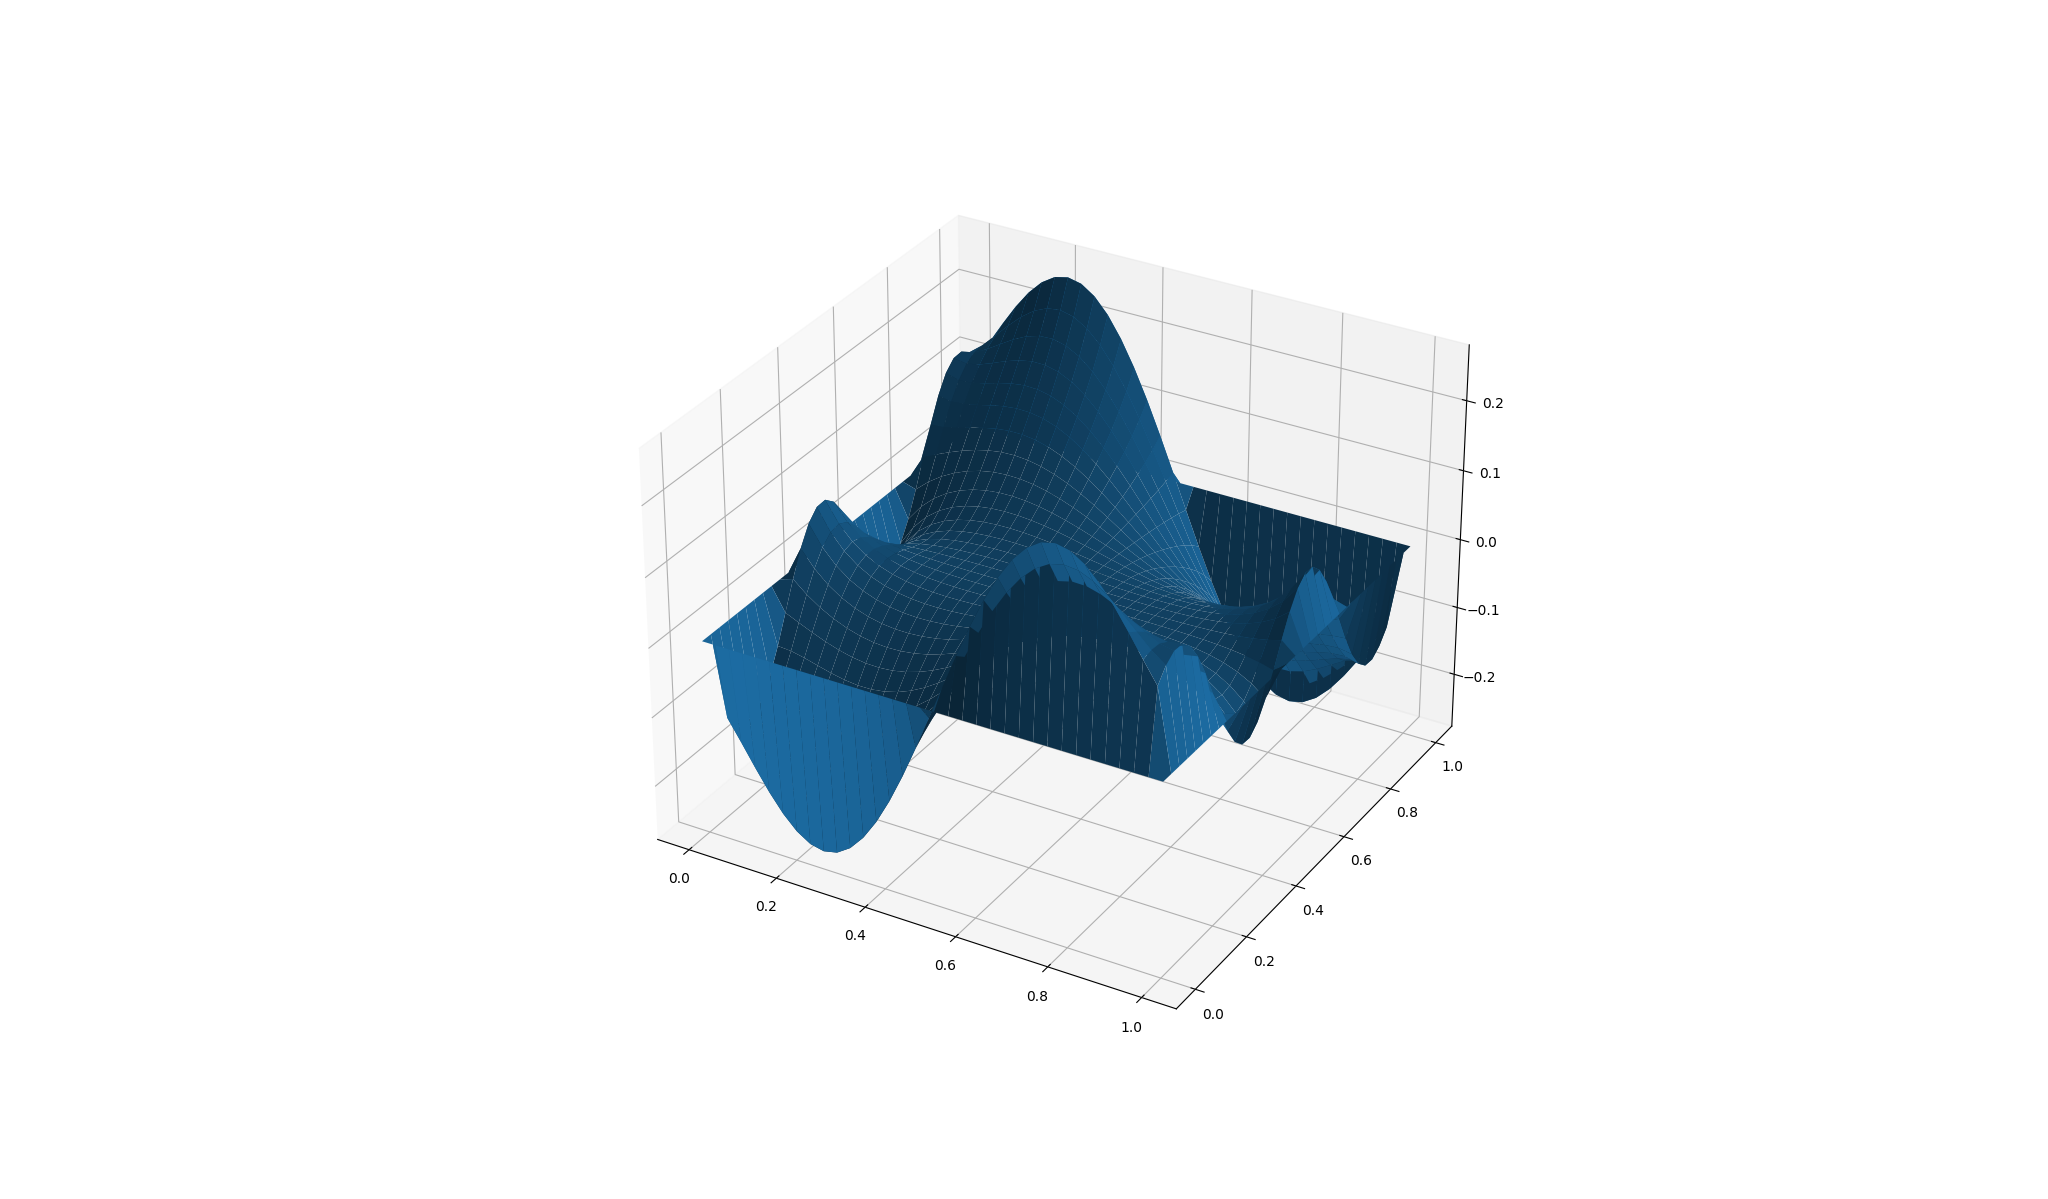
\includegraphics[width=0.35\textwidth]{problemThree/error.png}
		\caption{Difference of exact and approximate solution}
	\end{figure}
	Here is the code that generated these (\verb+laplace_zeroBC.py+).
	\lstinputlisting[language=Python]{problemThree/laplace_zeroBC.py}

	\subsubsection*{Heat Equation}
	First, the mesh/contour plots.
	\begin{figure}[h]
		\centering
		\begin{subfigure}{.5\textwidth}
			\centering
			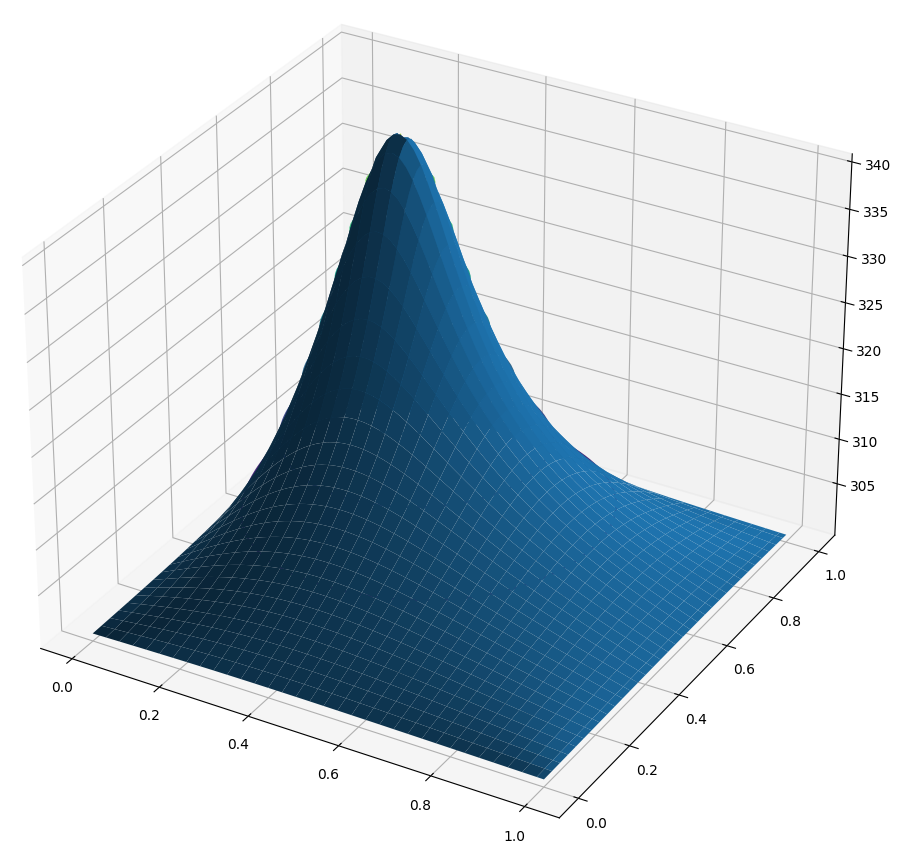
\includegraphics[width=.9\linewidth]{problemThree/heat_mesh.png}
			\caption{Mesh plot for heat equation}
			\label{fig:sub1}
		\end{subfigure}%
		\begin{subfigure}{.5\textwidth}
			\centering
			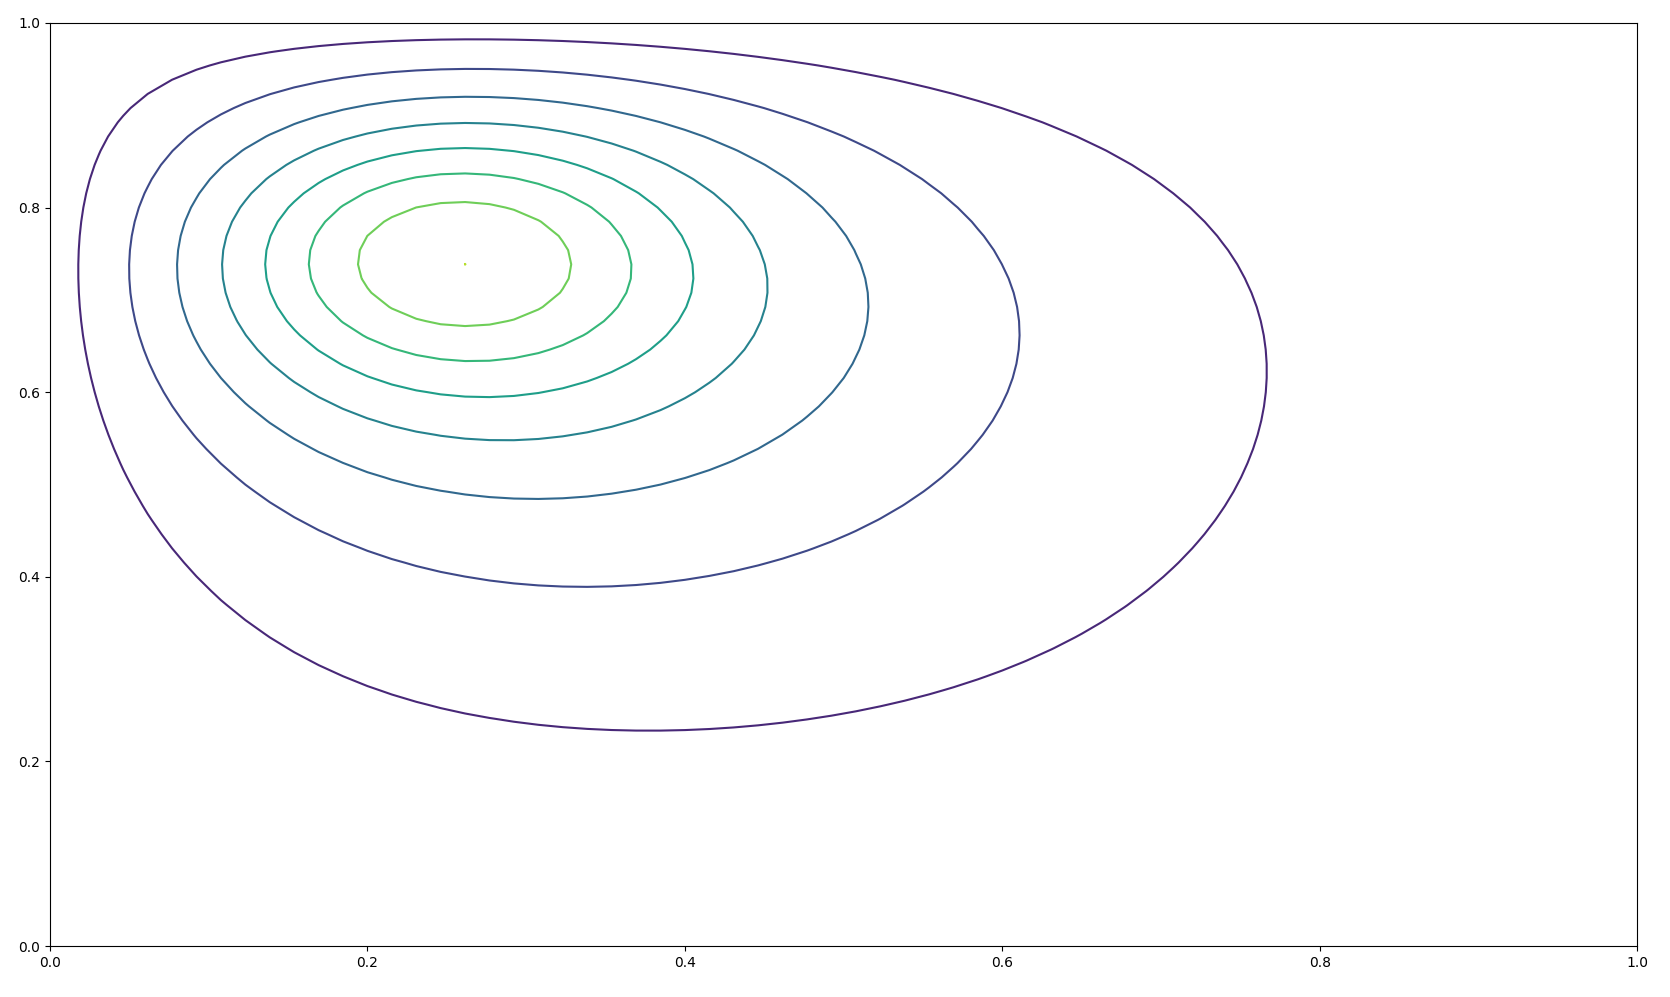
\includegraphics[width=.9\linewidth]{problemThree/heat_contour.png}
			\caption{Contour plot for heat equation}
			\label{fig:sub2}
		\end{subfigure}
	\end{figure}
	The maximum temperature is 340.0056172901325.

	The following code generated these (\verb+laplace_heat.py+).
	\lstinputlisting[language=Python]{problemThree/laplace_heat.py}

\end{solution}

\begin{problem}
Conditioning of linear systems.
\end{problem}

\begin{solution}
	\subsubsection*{(a)}
	We begin by showing $\kappa_2(A)$ is always equal to 1 if $A$ is an orthogonal matrix.
	\begin{equation}\label{eq:condition}
		\kappa_2(A) = \norm{A}_2\norm*{\inv{A}}_2
	\end{equation}
	We can expand these norms out as follows where we use $\inv{A} = \tpose{A}$ because for an orthogonal matrix $A\tpose{A} = \tpose{A}A = \mathbf{1}$.
	\begin{align*}
		\norm{A}_2^2 & = \lambda_\text{max}\qty(\tpose{A}A) & \norm*{\inv{A}}_2^2 & = \lambda_\text{max}\qty(\tpose{\qty(\inv{A})}\inv{A}) \\
		             & = \lambda_\text{max}\qty(\mathbf{1}) &                     & = \lambda_\text{max}\qty(A\tpose{A})                   \\
		             & = 1                                  &                     & = \lambda_\text{max}\qty(\mathbf{1}) = 1
	\end{align*}
	Plugging these two equations into \cref{eq:condition} we see $\kappa_2(A) = 1$ for all orthogonal $A$.

	\subsubsection*{(b)}
	Here we show the matrix $A = \smqty[1 & -1 \\ 1 & \phantom{-}1]$ is not orthogonal.
	\begin{equation*}
		A\tpose{A} = \mqty[1 & -1 \\ 1 & \phantom{-}1]\mqty[\phantom{-}1 & 1 \\ -1 & 1] = \mqty[2 & 0 \\ 0 & 2] = 2\mathbf{1} \neq \mathbf{1}
	\end{equation*}
	We can see here that $\inv{A} = \frac{1}{2}\tpose{A}$ which we will use below in our calculation of $\kappa_2(A)$.
	\begin{align*}
		\kappa_2(A) & = \norm{A}_2\norm*{\inv{A}}_2 = \sqrt{\lambda_\text{max}\qty(\tpose{A}A)}\sqrt{\lambda_\text{max}\qty(\tpose{\qty(\inv{A})}\inv{A})} \\
		            & = \sqrt{\lambda_\text{max}\qty(2\cdot\mathbf{1})}\sqrt{\tfrac{1}{4}\lambda_\text{max}\qty(A\tpose{A})}                               \\
		            & = \sqrt{2}\sqrt{\tfrac{1}{2}} = 1
	\end{align*}
	Because $\kappa_2(A) = 1$, we can conclude the matrix is well-conditioned.

	When computing the solution to the perturbed problem, the change in solution from the unperturbed problem is very small. This is because the matrix is well conditioned ($\kappa_2$ is small)

	\subsubsection*{(c)}
	First, is the matrix $B = \smqty[1 & -1 + \delta \\ 1 & -1]$ orthogonal?
	\begin{equation*}
		B\tpose{B} = \mqty[1 & -1 + \delta \\ 1 & -1]\mqty[1 & 1 \\ -1 + \delta & -1] = \mqty[1 + \qty(\delta - 1)^2 & 2 - \delta \\ 2 - \delta & 2] \neq \mathbf{1}
	\end{equation*}
	We conclude the matrix is not orthogonal. Via python we can calculate the matrix condition number to be $\kappa_2(B) = 39,999,947,698.45045$, and hence we conclude the matrix is not well conditioned.

	When computing the solution to the perturbed problem, the change in solution from the unperturbed problem is massive (on the order $10^6$). This is because the matrix is very ill conditioned ($\kappa_2$ is \emph{very} large).

	Below is the code I used to compute things for this question (\verb+conditioning.py+).
	\lstinputlisting[language=Python]{problemFour/conditioning.py}
	And here's what it outputs when run.
	\begin{verbatim}
--------------------------
------- P A R T  B -------
--------------------------
solution for unperturbed problem:
[[1.]
 [0.]]
matrix condition number: 1.0000000000000004
solution for perturbed problem:
[[ 1.0005e+00]
 [-5.0000e-04]]
relative condition number of perturbation: 1.0
--------------------------
------- P A R T  C -------
--------------------------
solution for unperturbed problem:
[[ 1.]
 [-0.]]
inverse of B:
[[ 9.99999917e+09 -9.99999917e+09]
 [ 9.99999917e+09 -9.99999917e+09]]
matrix condition number: 39999947698.45045
solution for perturbed problem:
[[10000000.17259526]
 [ 9999999.17259526]]
relative condition number of perturbation: 19999998345.19272
	\end{verbatim}
\end{solution}

\end{document}